\documentclass[12pt]{article}

\usepackage{amssymb,amsmath,amsbsy,amsfonts}
\usepackage{color}
\usepackage{epsfig}
\usepackage{fancybox,fancyhdr}
\usepackage{float}
\usepackage{framed}
\usepackage{fullpage}
\usepackage{graphicx}
\usepackage{listing}
\usepackage{listings}
\usepackage{shadow}
\usepackage{url}
\usepackage{version}
\usepackage{wrapfig}

\usepackage[T1]{fontenc}
\usepackage[utf8]{inputenc}
\usepackage[english, ngerman]{babel}
\usepackage{ae}

\lstset{
	literate=
		{ö}{{\"o}}1
		{Ö}{{\"O}}1
		{ä}{{\"a}}1
		{Ä}{{\"A}}1
		{ü}{{\"u}}1
		{Ü}{{\"U}}1
		{ß}{{ss}}1
}

\lstset{ %
	language=c,
	basicstyle=\footnotesize,
	numbers=left,
	numberstyle=\tiny,
	stepnumber=1,
	numbersep=5pt,
	backgroundcolor=\color{white},
	showspaces=false,
	showstringspaces=false,
	frame=single,
	showtabs=false,
	tabsize=2,
	captionpos=none,
	breaklines=true,
	breakatwhitespace=false,
	title=\lstname,
	escapeinside={\#}{\ },
	morekeywords={*,...}
}

\usepackage[
	pdftitle={Systemprogrammierung Dokumentation},
	bookmarks=true,
	bookmarksnumbered=true,
	colorlinks,
	linkcolor=red,
	urlcolor=blue,
	citecolor=black
]{hyperref}

\pagestyle{fancy}
\cfoot{}
\setlength{\topskip}{10mm}

\setcounter{tocdepth}{4}

\usepackage{color}
\definecolor{hellgrau}{gray}{0.9}
\definecolor{shadecolor}{gray}{0.9}

\newcommand{\ia}{i.\,Allg.\ }
\newcommand{\dht}{d.\,h.\ }
\newcommand{\ua}{u.\,a.\ }
\newcommand{\so}{s.\,o.\ }
\newcommand{\zb}{z.\,B.\ }
\newcommand{\zbdp}{z.\,B.:\ }
\newcommand{\idr}{i.\,d.\,R.\ }
\newcommand{\zt}{z.\,T.\ } 
\newcommand{\zz}{z.\,Zt.\ } 
\newcommand{\igs}{i.\,Ggs.\ } 

\newcommand{\code}[1]{\texttt{#1}}

\newcommand{\codeo}[2]{
\begin{shaded}
\vspace*{-2ex}
\begin{program}
\begin{leftbar}
                \label{def:#1}
                \rm #2
\end{leftbar}
\end{program}
\vspace*{-2ex}
\end{shaded}
}

\newcommand{\svs}{\vspace*{0.5ex}} 
\newcommand{\myrule}{\ \vspace{1ex} \\ \hrule} 
\newcommand{\figref}[1]{Abb.~\ref{#1}} 
\newcommand{\secref}[1]{Abschnitt~\ref{#1}} 
\newcommand{\mymargin}[1]{\marginpar{\raggedright \footnotesize \sffamily #1}} 

\renewcommand{\topfraction}{0.95}
\renewcommand{\bottomfraction}{0.95}

\newenvironment{trilist}{
    \renewcommand{\labelitemi}{\(\triangleright\)}
    \renewcommand{\labelitemii}{{\bfseries -}}
    \setlength{\partopsep}{0ex plus .5ex minus .5ex} 
    \setlength{\topsep}{-1ex plus .5ex minus .5ex} 
    \setlength{\parskip}{1.2ex plus .5ex minus .5ex}
    \setlength{\itemsep}{0pt plus .5ex minus .5ex}
    \setlength{\parsep}{0pt plus .5ex minus .5ex} 
    \begin{itemize}
    }
   {\end{itemize}}


\begin{document} 

	%Titelseite
\begin{titlepage}
\sffamily
\setlength{\tabcolsep}{0mm}
\begin{tabular*}{\textwidth}{l@{\extracolsep\fill}r} 

%\hspace{-0.4cm}
%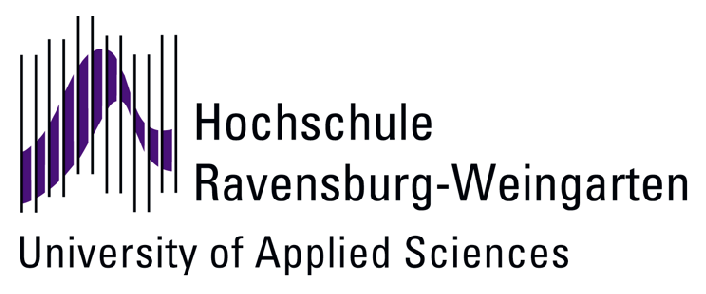
\includegraphics[width=6cm]{Bilder/logo_welle_en}  % Englische Version des Logos 

\includegraphics[width=5cm]{Bilder/logo_welle_de} % Deutsche Version des Logos

  &
\raisebox{3mm}{
	\begin{tabular}{r}
%\rule{0cm}{0.5cm}
Studiengang Angewandte Informatik\\[0.5mm]
Fakultät Elektrotechnik und Informatik \\
\end{tabular}}
\end{tabular*}
\setlength{\tabcolsep}{6pt}

\vspace*{4cm}
\begin{center}
\textbf{\Large{Dokumentation Gruppe 10}}\\
\vspace*{1cm}
\textbf{\LARGE{Systemprogrammierung}}\\
\vspace*{2cm}
%\large{zur Erlangung des akademischen Grades}\\[2mm]
%\large{Master of Science der Informatik}\\
\end{center}

%\vfill
\vspace{1cm}
\begin{center}

	vorgelegt von:\\[5mm]
	{\Large Frank Klameth} \\
	20688 \\
	frank.klameth@hs-weingarten.de \\[5mm]
	{\Large Simon Westphahl} \\
	20146 \\
	simon.westphahl@hs-weingarten.de \\[5mm]
	{\Large Michael Wydler} \\
	20168 \\
	michael.wydler@hs-weingarten.de \\[5mm]
    \today \\[3cm]
\end{center}

\end{titlepage}

\newpage


	\tableofcontents

	\section{Entwurf der Softwarekomponenten}


\subsection{Funktionalität Client}
Das Programm wird aus der Konsole gestartet. Es müssen folgende Parameter angegeben werden:
\begin{itemize}
	\item -s - Servername oder IP (Servername wird in IP umgewandelt)
	\item -p - Port\footnote{optional, wird sonst auf Default-Port (50000) gesetzt}
	\item -b - Benutzername
	\item -r - Rolle
\end{itemize}

Dabei können Benutzername und Rolle frei gewählt werden. Ist die angegebene Rolle schon belegt, wird der Benutzer automatisch als Student eingetragen.

\paragraph*{Beispiele: \\}
\code{> ./client 127.0.0.1 50100 michael student} \\
\code{> ./client 127.0.0.1 michael dozent}

\subsubsection{Hauptprogramm}
\begin{lstlisting}
# Start mit Parameter (Server-IP, Port, Username, Rolle)
# Socket für Netzwerkkommunikation öffnen
# Logindaten (Username und gewünschte Rolle) an Server senden
# Login erfolgreich?
    # wenn NEIN: 
        # Fehlermeldung ausgeben
        # Kill: Client
    # wenn JA:
        # Userdaten und -rechte speichern (ID, Name, Rechte)
# Mutex für lokalen Tafelzugriff initialisieren (gesperrt)
# Initialisiere lokale Tafel
# Starte Command-Thread
# Starte Live-Agent
# Starte GUI
# Starte Listener-Thread
# Starte Trigger für Live-Agent
    # Mutex-Down für lokale Tafel
    # Fordert aktuellen Tafelinhalt an
    # Mutex-Up
\end{lstlisting}

\subsubsection{Command-Thread}
\begin{lstlisting}
> quit (Client beenden)
    # Sende Befehl "quit" an den Server
    # Mutex-Down für lokale Tafel
    # Beende Trigger für Live-Agent
    # Kill: Listener-Thread
    # Kill: GUI
    # Kill: Live-Agent
    # Kill: Command-Thread
    # Lösche lokale Tafel
    # Lösche Mutex für Tafelzugriff
\end{lstlisting}
\begin{lstlisting}
> request (Schreibrecht anfordern)
    # Ist Client Student?
        # Wenn JA:
            # Sende Befehl "request" an den Server
    # Ist Client Dozent?
        # Wenn JA:
            # Dialog ob Benutzer schreibrecht bekommen soll
            # Sende Antwort an Server
    # Schreibrecht erteilt?
        # Wenn JA:
            # Deaktiviere Button 'Schreibrecht anfordern'
            # Aktiviere Button 'Schreibrecht abgeben'
            # Schreibrecht auf lokale Tafel gewähren
        # Wenn NEIN:
            # Hinweis das Anfrage abgeleht wurde.
\end{lstlisting}
\begin{lstlisting}
> shutdown (System beenden)
    # Ist Client Dozent?
        # Wenn JA:
            # Sende Befehl "shutdown" an den Server
\end{lstlisting}
\begin{lstlisting}
> release (Schreibrecht abgeben)
    # Ist Client Tutor?
        # Wenn JA:
            # Sende Befehl "release" an den Server
\end{lstlisting}
\begin{lstlisting}
> acquire (Schreibrecht entziehen)
    # Ist Client Dozent?
        # Wenn JA:
            # Sende Befehl "acquire" an den Server
\end{lstlisting}
\begin{lstlisting}
> clear (Tafel löschen)
    # Hat Client Schreibrechte?
        # Wenn JA:
            # Sende Befehl "clear" an den Server
\end{lstlisting}

\subsubsection{Live-Agent}
\begin{lstlisting}
> modify (Tafel ändern)
    # Hat Client schreibrecht?
        # Wenn JA:
            # Mutex-Down für lokale Tafel
            # Ist Tafel voll?
                # Wenn JA:
                    # Fehlermeldung
                # Wenn NEIN:
                    # Schreibe Änderung in lokale Tafel
            # Mutex-Up
            # Trigger für Tafel starten.
    # Trigger für Tafel sendet dann die Daten in bestimmten Intervallen.
    # Trigger abgelaufen?
        # Wenn JA:
            # Mutex-Down für lokale Tafel
            # Sende Tafel an Server
            # Erfolgreiche Sendung?
                # Wenn NEIN:
                    # Tafel nochmals senden
            # Mutex-Up
\end{lstlisting}

\subsubsection{Listener-Thread}
\begin{lstlisting}
> board_modified (Tafel-Update)
    # Mutex-Down für lokale Tafel
    # Tafel aktuallisieren
    # Mutex-Up
\end{lstlisting}
\begin{lstlisting}
> states_changed (Statusänderung)
    # GUI-Informationen aktuallisieren
\end{lstlisting}
\begin{lstlisting}
> my_state_changed (eigene Rechte bekommen/entzogen)
    # Schreibrecht erhalten?
        # Wenn JA:
            # Button "Schreibrecht anfordern" deaktivieren
            # Tafel editierbar setzten
    # Schreibrecht abgegeben/entzogen?
        # Wenn JA:
            # Tafel nicht-editierbar setzten
            # Button "Schreibrecht anfordern" aktivieren
\end{lstlisting}

\subsubsection{GUI}
\begin{lstlisting}
# // Tafel wird als GtkTextView gespeichert.
# GtkTextBuffer *gtkbuf = gtk_text_view_get_buffer(textview);

# GtkTextIter startIter, endIter;
# char *mybuf;

# gtk_text_buffer_get_start_iter(gtkbuf, &startIter);
# gtk_text_buffer_get_end_iter(gtkbuf, &endIter);

# // Speichern in char*
# mybuf = gtk_text_buffer_get_text(gtkbuf, &startIter, &endIter, FALSE);

# // Tafel leeren
# gtk_text_buffer_set_text(gtkbuf, "", -1);

# // Tafel wieder befüllen
# gtk_text_buffer_set_text(gtkbuf, mybuf, -1);
\end{lstlisting}

\subsubsection{Tafel-Trigger}
Wenn auf die Tafel geschrieben wird, dann wird ein Timeout-Signal gestartet. Wenn dieses abgelaufen ist, wird die Tafel an den Server gesendet und somit an alle Clients verteilt.
Bei jeder Änderung wird der Timeout zurückgesetzt. Wenn der Timeout 5x zurückgesetzt wurde, dann wird die Tafel dennoch zum Server gesendet und der Timeout-Counter zurückgesetzt.
\begin{lstlisting}
# Tafel wird geändert
    # Timeout (200ms) wird (neu) gestartet
    # Timeout-Counter +1
    # Timeout abgelaufen oder Timeout-Counter = 3?
        # Wenn JA:
            # Mutex-Down für lokale Tafel
            # Tafel an Server senden
            # Timeout-Counter = 0
            # Mutex-Up
\end{lstlisting}


\subsection{Funktionalität Server}
Das Programm wird aus der Konsole gestartet. Es können folgende Parameter angegeben werden:
\begin{itemize}
	\item -p - Port\footnote{optional, sonst wird Default-Port (50000) benutzt.}
	\item -d - Debugging-Mode (ohne Argument)
\end{itemize}

\paragraph*{Beispiele: \\}
\code{> ./server -p 8080 -d} \\
\code{> ./server}

\subsubsection{Hauptprogramm}
\begin{lstlisting}
# Sicherstellen, dass noch kein Server läuft
# Mutex für Tafelzugriff initialisieren (gesperrt)
# Mutex für Zugriff auf Client-Liste initialisieren (gesperrt)
# Initialisierung der Tafel (Shared Memory)
# Initialisierung der Client-Liste (doppelt verkettete Liste)
# Initialisierung Semaphore (Zähler) für aktive Clients (*** GEEIGNET??? ***)
# Message Queue für Logging initialisieren
# Initialisiere Trigger für Broadcasting-Agent (*** IMPLEMENTIERUNG??? ***)
# Initialisiere Trigger "Tafel archiviert" (Condition Variable > pthread)
# Signal registrieren für "System beenden"
# Socket für Netzwerkkommunikation öffnen

# Fork: Logger (externes Programm)
# Fork: Archivierer (externes Programm), wenn Debugmodus mit Archivierungsintervall
# Starte Broadcasting-Agent als Thread
# Starte Login-Thread
# Mutex für Tafelzugriff freigeben
# Mutex für Clientliste freigeben
\end{lstlisting}

\subsubsection{Signal System beenden}
\begin{lstlisting}
# Mutex-Down: Clientliste
    # Kill: Login-Thread
# Mutex-Up: Clientliste
# Trigger Broadcasting Agent: Clients beenden (quit)
# Warte auf Sempahore (Clientzähler) == 0 (*** GEEIGNET??? ***)
    # Kill: Broadcasting Agent
# Netzwerksocket schließen
# Kill: Archivierer
# Kill: Logger
# Message Queue (Logger) löschen
# Mutex-Down: Tafel
# Freigabe: Shared Memory (Tafel)
\end{lstlisting}

\subsubsection{Login-Thread}
\begin{lstlisting}
# Warte auf Login von Client
# Mutex-Down für Zugriff auf Client-Liste 
    # Prüfung: Clientname bereits in Liste?
        # wenn Ja: Fehlermeldung an Client
    # Schreibrecht: Nein
    # Wenn Rolle Dozent: Prüfung, bereits ein Dozent angemeldet?
        # wenn Ja: ändere Rolle Dozent -> Student
        # wenn Nein: Schreibrecht zuweisen
    # Wenn Rolle Tutor: ändere Rolle zu Student
    # (IP/DNS-Name,) Client-Name, Rolle + Zugriffsrecht in Liste eintragen
    # Semaphore (Clientzähler) Up
# Mutex-Up für Zugriff auf Client-Liste
# Starte Client-Thread für neuen Client
# Trigger Broadcasting-Agent: Update Anzahl Clients
\end{lstlisting}

\subsubsection{Client-Threads}
\begin{lstlisting}
# Rückmeldung an Client: Login erfolgreich
# Warte auf Befehle von verbundenem Client
> quit (Client beenden) bzw. Client schließt Verbindung
    # Mutex-Down für Zugriff auf Client-Liste
        # Client aus Client-Liste austragen
        # Semaphore (Client-Zähler) Down
    # Mutex-Up
    # Trigger Broadcasting-Agent: Sende neue Clientanzahl
    # Tread beenden
\end{lstlisting}
\begin{lstlisting}
> request (Schreibrechte anfordern)
    # Mutex-Down für Zugriff auf Client-Liste
        # hat Client bereits schreibrecht bzw. ist Dozent?
            # wenn Ja: Fehlermeldung
        # suche Dozent in Clientliste
            # kein Dozent: Fehlermeldung
    # Mutex-Up
    # Anfrage für Schreibrecht an Dozent
    # Warte auf Antwort von Dozent
        # Antwort Nein: Fehlermeldung an anfragenden Benutzer
    # Mutex-Down für Zugriff auf Client-Liste
        # setze alter Benutzer mit Schreibrechten: keine Schreibrechte
        # aktueller Benutzer: Schreibrecht
    # Mutex-Up
    # Statusänderung alter Benutzer: keine Schreibrechte
    # Statusänderung anfragender Benutzer: Schreibrechte    
    # Trigger Broadcasting-Agent: Tutor = 1
\end{lstlisting}
\begin{lstlisting}
> shutdown
    # Mutex-Down für Zugriff auf Client-Liste
        # Benuter ist Dozent?
            # wenn Nein: Fehlermeldung
    # Mutex-Up
    # Signal senden: System beenden
\end{lstlisting}
\begin{lstlisting}
> release
    # Mutex-Down für Zugriff auf Client-Liste
        # Benutzer ist Tutor?
            # wenn Nein: Fehlermeldung
        # aktueller Benutzer: Schreibrecht > Nein
        # ändere Rolle Tutor -> Student
        # Dozent: Schreibrecht Ja
    # Mutex-Up
    # Trigger Broadcasting-Agent: Tutoren = 0
    # Sende Statusänderung Dozent: Schreibrecht erhalten
\end{lstlisting}
\begin{lstlisting}
> acquire
    # Mutex-Down für Zugriff auf Client-Liste
        # aktueller Benutzer ist Dozent?
            # wenn Nein: Fehlermeldung
        # entziehe Tutor Schreibrecht
        # setze Dozent Schreibrecht
    # Mutex-Up
    # Statusänderung vorheriger Tutor: keine Schreibrechte
    # Trigger Broadcasting-Agent: Tutoren = 0
    # Sende Statusänderung Dozent: Schreibrechte
\end{lstlisting}
\begin{lstlisting}
> modify
    # Mutex-Down für Zugriff auf Client-Liste
        # Benutzer hat Schreibrechte?
            # wenn Nein: Fehlermeldung
    # Mutex-Up
    # Mutex-Down für Zugriff auf Tafel
        # Änderungen in Shared Memory schreiben
    # Mutex-Up
    # Trigger Broadcasting-Agent: Tafeländerung
\end{lstlisting}
\begin{lstlisting}
> clear
    # Mutex-Down für Zugriff auf Client-Liste
        # Benutzer hat Schreibrechte?
            # wenn Nein: Fehlermeldung
    # Mutex-Up
    # Mutex-Down für Zugriff auf Tafel
    # Trigger Archivierer
        *** Im Archivierer ist kein Mutex-Down notwendig. Dies erfolgt vor
        *** der Triggerung des Archivierers, um sicherzustellen, das in der
        *** Zwischenzeit niemand anders auf die Tafel zugreift.
        *** Der Archivierer macht nach dem Sichern der Tafel einen Mutex-Up
    # Mutex-Down für Zugriff auf Tafel
        # Lösche Tafel  
    # Mutex Up
    # Trigger Broadcasting-Agent: Tafel leer
\end{lstlisting}

\subsubsection{Broadcasting-Agent}
\begin{lstlisting}
# Warte auf Trigger
# Wenn Tafeländerung
    # Mutex-Down für Zugriff auf Tafel
        # Lese Tafelinhalt
    # Mutex-Up
# Sende Nachricht an alle verbundenen Clients
\end{lstlisting}


\subsection{Funktionalität Logger}
\begin{lstlisting}
# Öffne Message Queue
# Warte auf Messages
# Schreibe Zeitstempel + Nachricht in Datei (zeilenweise)
\end{lstlisting}


\subsection{Funktionalität Archivierer}
\begin{lstlisting}
# Öffne Logfile (schreibbar)
# Warte auf Trigger bzw. Ablauf von Timer (Debug-Modus)
# Ausgelöst durch Timer?
    # wenn Ja: Mutex
    *** Vor dem Auslesen der Tafel ist nur ein Mutex-Down notwendig, wenn
    *** der Auslöser für die Archivierung durch den Timer erfolgt ist.
    *** Andernfalls ist dies bereits durch den Client-Thread geschehen um
    *** sicherzustellen, dass der Tafelinhalt erst nach dem Archivieren
    *** gelöscht wird.
# Tafel auslesen
# Mutex-Up
# Zeitstempel + Tafelinhalt in Datei schreiben (blockweise)
\end{lstlisting}


\subsection{Synchronisationsprotokoll}
siehe Petrinetz.

\subsection{Netzwerkschnittstellen}

\subsubsection{Header}
\myfigure{Header}{header.pdf}
\begin{tabular}{ll}
Type & uint8\_t \\
Lenght & uint16\_t
\end{tabular}

\subsubsection{Login}
\myfigure{Login}{login.pdf}

\subsubsection{Tafelinhalt}
\myfigure{Tafelinhalt}{board_content.pdf}

\subsubsection{Tafel löschen}
\myfigure{Tafel löschen}{clear_board.pdf}

\subsubsection{Schreibrechtanfrage}
\myfigure{Schreibrechtanfrage C -> S}{write_request.pdf}

\myfigure{Schreibrechtanfrage S -> D}{write_requested.pdf}

\myfigure{Schreibrechtanfrage D -> S}{request_reply.pdf}

\subsubsection{Beenden}
\myfigure{Beenden}{shutdown.pdf}

\subsubsection{Status-Nachricht}
\myfigure{Status-Nachricht}{status_nachricht.pdf}

\subsubsection{Fehlernachricht}
\myfigure{Fehlernachticht}{error_message.pdf}
 
	\section{Client}
Der Client stellt eine Verbindung zum Server her. Es werden bein starten des Client die Server- und Logindaten angegeben.

\subsection{Module}
\begin{itemize}
	\item Login
	\item Benutzeroberfläche (GUI)
	\item Live-Agent
	\item Listener-Thread
	\item Netzwerkkommunikation
	\begin{itemize}
		\item Struct vor Senden Serialisieren
		\item Nach Empfang wieder umwandeln
	\end{itemize}
\end{itemize}

\subsection{Programmstart}
Das Programm wird aus der Konsole gestartet. Es müssen folgende Parameter angegeben werden:
\begin{itemize}
	\item Servername oder IP (Servername wird in IP umgewandelt)
	\item Port
	\item Benutzername
	\item Rolle
\end{itemize}

Dabei können Benutzername und Rolle frei gewählt werden. Ist der Benutzername schon vergeben, wird ... . Ist die angegebene Rolle schon belegt, wird der Benutzer automatisch als Student eingetragen.

\paragraph{Beispiel:}
\code{> ./client 127.0.0.1 8080 michael student}

\subsection{Strukturen (intern)}
\subsubsection{Benutzerrollen}
\begin{lstlisting}
enum ROLE {
    Dozent = 1
    Tutor = 2
    Student = 3
};
\end{lstlisting}

\subsubsection{Schreib- und Leserecht}
Als Datentyp wird \code{uint8\_t} verwendet.
\begin{itemize}
	\item Modify 0 = nur lesend
	\item Modify 1 = schreibzugriff (exclusiv)
\end{itemize}

\subsection{Abläufe \label{Abläufe}}

\subsubsection{Programmstart}
\begin{lstlisting}
# Start mit Parameter (Server-IP, Port, Username, Rolle)
# Socket für Netzwerkkommunikation öffnen
# Logindaten (Username und gewünschte Rolle) an Server senden
# Login erfolgreich?
    # wenn NEIN: 
        # Fehlermeldung ausgeben
        # Kill: Client
    # wenn JA:
        # Userdaten und -rechte speichern (ID, Name, Rechte)
# Mutex für lokalen Tafelzugriff initialisieren (gesperrt)
# Initialisiere lokale Tafel
# Starte Command-Thread
# Starte Live-Agent
# Starte GUI
# Starte Listener-Thread
# Starte Trigger für Live-Agent
    # Mutex-Down für lokale Tafel
    # Fordert aktuellen Tafelinhalt an
    # Mutex-Up
\end{lstlisting}

\subsubsection{Command-Thread}
\begin{lstlisting}
> quit (Client beenden)
    # Sende Befehl "quit" an den Server
    # Mutex-Down für lokale Tafel
    # Beende Trigger für Live-Agent
    # Kill: Listener-Thread
    # Kill: GUI
    # Kill: Live-Agent
    # Kill: Command-Thread
    # Lösche lokale Tafel
    # Lösche Mutex für Tafelzugriff

> request (Schreibrecht anfordern)
    # Ist Client Student?
        # Wenn JA:
            # Sende Befehl "request" an den Server
    # Ist Client Dozent?
        # Wenn JA:
            # Dialog ob Benutzer schreibrecht bekommen soll
            # Sende Antwort an Server
    # Schreibrecht erteilt?
        # Wenn JA:
            # Deaktiviere Button 'Schreibrecht anfordern'
            # Aktiviere Button 'Schreibrecht abgeben'
            # Schreibrecht auf lokale Tafel gewähren
        # Wenn NEIN:
            # Hinweis das Anfrage abgeleht wurde.

> shutdown (System beenden)
    # Ist Client Dozent?
        # Wenn JA:
            # Sende Befehl "shutdown" an den Server

> release (Schreibrecht abgeben)
    # Ist Client Tutor?
        # Wenn JA:
            # Sende Befehl "release" an den Server

> acquire (Schreibrecht entziehen)
    # Ist Client Dozent?
        # Wenn JA:
            # Sende Befehl "acquire" an den Server

> clear (Tafel löschen)
    # Hat Client Schreibrechte?
        # Wenn JA:
            # Sende Befehl "clear" an den Server
\end{lstlisting}

\subsubsection{Live-Agent}
\begin{lstlisting}
> modify (Tafel ändern)
    # Hat Client schreibrecht?
        # Wenn JA:
            # Mutex-Down für lokale Tafel
            # Ist Tafel voll?
                # Wenn JA:
                    # Fehlermeldung
                # Wenn NEIN:
                    # Schreibe Änderung in lokale Tafel
            # Mutex-Up
            # Trigger für Tafel starten.
    # Trigger für Tafel sendet dann die Daten in bestimmten Intervallen.
    # Trigger abgelaufen?
        # Wenn JA:
            # Mutex-Down für lokale Tafel
            # Sende Tafel an Server
            # Erfolgreiche Sendung?
                # Wenn NEIN:
                    # Tafel nochmals senden
            # Mutex-Up
\end{lstlisting}

\subsubsection{GUI}
\begin{lstlisting}
# // Tafel wird als GtkTextView gespeichert.
# GtkTextBuffer *gtkbuf = gtk_text_view_get_buffer(textview);

# GtkTextIter startIter, endIter;
# char *mybuf;

# gtk_text_buffer_get_start_iter(gtkbuf, &startIter);
# gtk_text_buffer_get_end_iter(gtkbuf, &endIter);

# // Speichern in char*
# mybuf = gtk_text_buffer_get_text(gtkbuf, &startIter, &endIter, FALSE);

# // Tafel leeren
# gtk_text_buffer_set_text(gtkbuf, "", -1);

# // Tafel wieder befüllen
# gtk_text_buffer_set_text(gtkbuf, mybuf, -1);
\end{lstlisting}

\subsubsection{Listener-Thread}
\begin{lstlisting}
# Wartet auf Nachrichten vom Server (Broadcasting-Thread)
# Aktuallisierung der lokalen Tafel und der Statusinformationen.

> board_modified (Tafel-Update)
    # Mutex-Down für lokale Tafel
    # Tafel aktuallisieren
    # Mutex-Up

> states_changed (Statusänderung)
    # GUI-Informationen aktuallisieren

> my_state_changed (eigene Rechte bekommen/entzogen)
    # Schreibrecht erhalten?
        # Wenn JA:
            # Button "Schreibrecht anfordern" deaktivieren
            # Tafel editierbar setzten
    # Schreibrecht abgegeben/entzogen?
        # Wenn JA:
            # Tafel nicht-editierbar setzten
            # Button "Schreibrecht anfordern" aktivieren
\end{lstlisting}

\subsection{Tafel-Trigger}
Wenn auf die Tafel geschrieben wird, dann wird ein Timeout-Signal gestartet. Wenn dieses abgelaufen ist, wird die Tafel an den Server gesendet und somit an alle Clients verteilt.
Bei jeder Änderung wird der Timeout zurückgesetzt. Wenn der Timeout 5x zurückgesetzt wurde, dann wird die Tafel dennoch zum Server gesendet und der Timeout-Counter zurückgesetzt.
\begin{lstlisting}
# Tafel wird geändert
    # Timeout (200ms) wird (neu) gestartet
    # Timeout-Counter +1
    # Timeout abgelaufen oder Timeout-Counter = 3?
        # Wenn JA:
            # Mutex-Down für lokale Tafel
            # Tafel an Server senden
            # Timeout-Counter = 0
            # Mutex-Up
\end{lstlisting}


	\section{Server}

\subsection{Programmabläufe}

\subsubsection{Hauptprogramm}
\myfigure{Ablauf Hauptprogramm}{ablaeufe/server/server_ablauf.pdf}{0.5}

\subsubsection{Login-Thread}
\myfigure{Ablauf Login-Thread}{ablaeufe/server/login_thread_ablauf.pdf}{0.5}

\subsubsection{Client-Thread}
\myfigure{Ablauf Client-Thread}{ablaeufe/server/client_thread_ablauf.pdf}{0.35}

\subsubsection{Broadcasting-Agent}
\myfigure{Ablauf Broadcasting-Agent}{ablaeufe/server/broadcasting_thread_ablauf.pdf}{0.5}

\subsection{Funktionshierarchie}
\myfigure{Funktionshierarchie Server}{hierarchie/server.pdf}{0.45}

\subsection{Modulhierarchie}
\myfigure{Modulhierarchie Server}{module/server/server_module.pdf}{0.65}

\subsection{Quellcode}
Der Quellcode ist auf der CD zu finden.

	\section{Logger}

\subsection{Programmablauf}
\begin{lstlisting}
# Öffne Message Queue
# Warte auf Messages
# Schreibe Zeitstempel + Nachricht in Datei (zeilenweise)
\end{lstlisting}

\subsection{Funktionshierarchie}

\subsection{Modulhierarchie}

\subsection{Quellcode}
Der Quellcode ist auf der CD zu finden.

	\section{Archivierer}

\subsection{Programmablauf}
\begin{lstlisting}
# Öffne Logfile (schreibbar)
# Warte auf Trigger bzw. Ablauf von Timer (Debug-Modus)
# Ausgelöst durch Timer?
    # wenn Ja: Mutex
    *** Vor dem Auslesen der Tafel ist nur ein Mutex-Down notwendig, wenn
    *** der Auslöser für die Archivierung durch den Timer erfolgt ist.
    *** Andernfalls ist dies bereits durch den Client-Thread geschehen um
    *** sicherzustellen, dass der Tafelinhalt erst nach dem Archivieren
    *** gelöscht wird.
# Tafel auslesen
# Mutex-Up
# Zeitstempel + Tafelinhalt in Datei schreiben (blockweise)
\end{lstlisting}

\subsection{Funktionshierarchie}

\subsection{Modulhierarchie}

\subsection{Quellcode}
Der Quellcode ist auf der CD zu finden.

	\section{Client-Liste}

\subsection{Datenstrukturen}
Die Daten von jedem Client wird in der Struktur \code{client\_data} gespeichert. 
Diese einzelnen Datenstrukturen werden dann in einer doppelt verketteten Liste gespeichert.
\begin{lstlisting}
struct client_data {
	uint16_t cid;
	int sfd;
	uint8_t role;
	char name[];
}
\end{lstlisting}
\begin{lstlisting}
struct cl_entry {
	struct client_data *cdata;
	struct cl_entry *next;
	struct cl_entry *previous;
}
\end{lstlisting}

\subsection{Exportierte Funktionen}
\begin{lstlisting}
void lock_clientlist ()
void unlock_clientlist ()
void add_client (struct client_data *cdata)
int remove_client (int sfd)
int docent_exists ()
int tutor_exists ()
struct cl_entry *get_write_user ()
void set_write_user (struct cl_entry *user)
struct cl_entry *get_docent ()
struct cl_entry *get_user_sfd (int sfd)
struct cl_entry *get_user_cid (uint16_t cid)
int has_write_access (int sfd)
int is_docent (int sfd)
uint16_t get_next_cid (void)
int get_client_count (void)
struct cl_entry *start_iteration ()
struct cl_entry *iteration_next ()
void end_iteration ()
\end{lstlisting}

	


	\section{Zusammenfassung und Fazit}

Das Praktikum 'Systemprogrammierung' hat uns einen tieferen Einblick in die
systemnahme Programmierung von Client-Server-Anwendungen gegeben. \\
Beim ersten Systementwurf war uns (und vielen anderen) nicht genau klar,
was gewünscht war und vor allem wie man das Problem angehen sollte.
Eine Verknüpfung mit der Vorlesung 'Software-Engineering' wäre hier wünschenswert
und hilfreicht gewesen. Desweiteren ist das Verhältnis von Arbeitsaufwand zu
Credits um ein vielfaches Höher als in anderen Praktikas bzw. Vorlesungen. \\
Die selbstständige Problemlösung war ein wichtiger Bestandteil aus dem wir
viel lernen konnten. Außerdem war das Praktikum eine gute Möglichkeit,
die theoretischen Kenntnisse aus der Vorlesung 'Betriebssysteme' praktisch
anzuwenden.

	%\section{Netzwerk}

\subsection{Allgemeine Definitionen}
\subsubsection{Datentypen}
Um hohe portabliltät zu gewährleisten verwenden wir nur sichere Datentypen.
Insbesondere gilt dies für Zahlen. Statt den Datentypen short, int, long verwenden
wir (u)int8\_t, (u)int16\_t, ....\\
Außerdem sollten immer Funktionen mit Längenbegrenzung benutzt werden, 
um Buffer-Overflows zu vermeiden.

\begin{figure}[ht!]
 \centering
 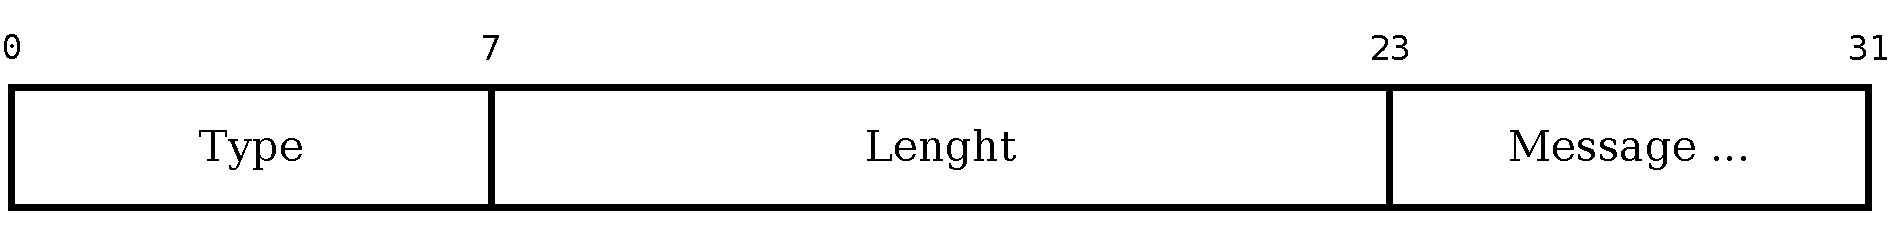
\includegraphics[width=\textwidth,keepaspectratio=true]{Bilder/header.pdf}
 \caption{Header}
 \label{Header}
\end{figure}

\subsubsection{Serialisierung}
Alle structs werden zum senden serialisiert in ein char-Array. \\
Der Server deserialisiert diesen String wieder.

\begin{lstlisting}
// PSEUDOCODE!
struct login_data {
    char name[50];
    uint8_t role;
}

// BUFFER
char buf[sizeof(login_data);

// SERIALISIEREN
strncpy(buf, login_data, sizeof(buf));

// DESERIALISIEREN
strncpy(login_data, buf, sizeof(login_data));
\end{lstlisting}

\subsubsection{Benutzerrollen}
\begin{lstlisting}
enum ROLE {
    Dozent = 1
    Tutor = 2
    Student = 3
};
\end{lstlisting}

\subsubsection{Schreib- und Leserecht}
Als Datentyp wird \code{uint8\_t} verwendet.
\begin{itemize}
	\item Modify 0 = nur lesend
	\item Modify 1 = schreibzugriff (exclusiv)
\end{itemize}

\subsubsection{Message-Types}
\begin{lstlisting}
enum M_TYPES {
    Login = 1,
    Quit, /*** eigentlich nicht nötig; Client bzw. Server */
          /*** schließt Verbindung einfach */
    Request,
    Shutdown,
    Release,
    Aquire,
    Modify,
    Clear,
    Status,
};
\end{lstlisting}

\subsection{Kommunikationsablauf}
Dieser Abschnitt spezifiziert den Austausch der einzelnen Datenstrukturen
über das Netzwerk.

Für die Beschreibung des Aufbaus der einzelnen Pakete: 
> siehe Abschnitt Datenstrukturen

\subsubsection{Login}
\begin{lstlisting}
Login       >>>
            <<<     Login
\end{lstlisting}

\subsubsection{Quit}
\begin{lstlisting}
*** eigentlich nicht nötig; Client bzw. Server schließt Verbindung einfach ***
\end{lstlisting}

\subsubsection{Request}
\begin{lstlisting}
Request     >>>
            <<<     Request (an Dozent)
# Bei Zustimmung des Dozenten die Schreibrechte abzugeben
Status      >>>
            <<<     Status (an anfragenden Client: Schreibrechte)
            <<<     Status (an alle Anderen: Tutor +1)
\end{lstlisting}

\subsubsection{Shutdown}
\begin{lstlisting}
Shutdown    >>>     (Server schließt alle Verbindungen)
\end{lstlisting}

\subsubsection{Release}
\begin{lstlisting}
Release     >>>
            <<<     Status (an releasing Client: nur Leserechte)
            <<<     Status (an Dozent: Schreibrechte)
            <<<     Status (an alle Anderen: Tutoren -1)
\end{lstlisting}

\subsubsection{Aquire}
\begin{lstlisting}
Aquire      >>>
            <<<     Status (an Client der aktuell schreibberechtig ist: nur lesend)
            <<<     Status (an Dozent: Schreibrechte)
            <<<     Status (an alle Anderen: Tutoren -1)
\end{lstlisting}

\subsubsection{Modify}
\begin{lstlisting}
Modify      >>>
            <<<     Modify (Änderungen an alle Clients verteilen)
\end{lstlisting}

\subsubsection{Clear}
\begin{lstlisting}
Clear       >>>
            <<<     Clear (an alle Clients: Tafel wurde gelöscht)
\end{lstlisting}

\subsubsection{Status}
\begin{lstlisting}
*** Ein eigener Status-Befehl existiert nicht. Status-Nachrichten
*** dienen als Bestätigung für bestimmte Befehle an den Client
*** und als Update für den Client-Status.
*** Für die Verwendung: siehe andere Befehle
\end{lstlisting}

\subsection{Datenstrukturen}
\begin{lstlisting}
#pragma pack(1)
struct HEADER {
    uint16_t size; /* Gesamtgröße in Bytes */
    uint8_t type; /* Wert aus M_TYPES */
};


/*
 * Packet:  Login
 *
 * Beschreibung:
 * Login-Versuch von Client bzw. Antwort von Server auf Login von Client.
 *
 *      >>> Richtung: Client > Server
 *      + "client_name" MUSS gesetzt und 0-terminiert sein und
 *        ist auf 25 Zeichen (inkl. O-Byte) begrenzt
 *      + "role" SOLLTE gesetzt sein, kann aber in jedem Fall vom
 *        Server geändert werden
 *
 *      >>> Richtung: Server > Client
 *      + "client_name" KANN gesetzt sein
 *      + wenn vorhanden muss dieser 0-terminiert sein und
 *        ist auf 25 Zeichen (inkl. 0-Byte) begrenzt
 *      + "role" MUSS gesetzt sein und MUSS vom Client respektiert werden
 *      + im Fehlerfall ist role == 0
 */
struct LOGIN {
    struct NET_HEADER header;
    char[25] client_name;
    uint8_t role; /* Wert aus ROLE */
};


/*
 * Packet:  Quit
 *
 * Beschreibung:
 * *** eigentlich nicht nötig; Client bzw. Server 
 * *** schließt Verbindung einfach
 *
 *      >>> Richtung: Server > Client
 *      + Keine Nutzdaten/Payload
 *      + Message Type in header ausreichend (kein "Payload Struct")
 */


/*
 * Packet:  Request
 *
 * Beschreibung:
 * Client fordert Schreibrechte an bzw. Anfrage an Dozent für Schreibrechte
 *
 *      >>> Richtung: Client > Server
 *      + "cid" wird nicht berücksichtigt
 *      + "client_name" KANN gesetzt sein
 *      + "client_name" muss 0-terminiert sein und ist auf 25 Zeichen
 *        begrenzt (inkl. 0-Byte)
 *
 *      >>> Richtung: Server > Client
 *      + "cid" MUSS gesetzt sein
 *      + "client_name" MUSS gesetzt sein
 *      + "client_name" MUSS 0-terminiert sein und ist auf 25 Zeichen
 *        begrenzt (inkl. 0-Byte)
 */
struct REQUEST {
    struct NET_HEADER header;
    uint8_t cid;
    char client_name[25];
};


/* 
 * Packet:  Shutdown
 *
 * Beschreibung:
 * System komplett beenden
 *
 *      >>> Richtung: Client > Server
 *      + Keine Nutzdaten/Payload
 *      + Message Type in header ausreichend (kein "Payload Struct")
 */


/*
 * Packet:  Release
 *
 * Beschreibung:
 * Schreibrechte an Dozent zurückgeben
 *
 *      >>> Richtung: Client > Server
 *      + Keine Nutzdaten/Payload
 *      + Message Type in header ausreichend (kein "Payload Struct")
 */


/*
 * Packet:  Aquire
 *
 * Beschreibung:
 * Aktuellem Benutzer Schreibrechte entziehen
 *
 *      >>> Richtung: Client > Server
 *      + Keine Nutzdaten/Payload
 *      + Message Type in header ausreichend (kein "Payload Struct")
 *
 */


/*
 * Packet:  Modify
 *
 * Beschreibung:
 * Änderungen an der Tafel übertragen
 *
 *		>>> Richtung: Client > Server
 *      + "cid" MUSS gesetzt sein
 *      + "board" MUSS gesetzt sein, ist 0-terminiert und max. 1200 Zeichen (inklusive 0-Byte)
 *
 *      >>> Richtung: Server > Client
 *      + "cid" wird nicht berücksichtigt
 *      + "board" MUSS gesetzt sein, ist 0-terminiert und max. 1200 Zeichen (inklusive 0-Byte)
 */
struct MODIFY {
    struct NET_HEADER header;
    uint8_t cid;
    char board[1200];
};


/*
 * Packet:  Clear
 *
 * Beschreibung:
 * Löschen des Tafelinhalts
 *
 *      >>> Richtung: Client > Server
 *      + Keine Nutzdaten/Payload
 *      + Message Type in header ausreichend (kein "Payload Struct")
 */


/*
 * Packet:  Status
 *
 * Beschreibung:
 * Änderung des Status im Server bzw. Client
 *
 *      Richtung: Client > Server (als Antwort auf 'Request'
 *      + "client_name" KANN gesetzt sein (vom Server nicht berücksichtigt)
 *      + "cid" MUSS gesetzt sein
 *      + restliche Elemente KÖNNEN gesetzt sein,
 *        aber vom Server nicht weiter berücksichtigt
 *
 *      Richtung: Server > Client
 *      + "client_name" MUSS gesetzt sein
 *      + "role" KANN gesetzt sein
 *      + "cid" KANN gesetzt sein
 *      + "write" MUSS entweder 1 = schreibender, oder 0 = lesender
 *        Zugriff sein
 *      + "nof_doz" (Anzahl angemeldeter Dozenten) KANN gesetzt sein
 *        und ist entweder 0 oder 1 (nicht mehr als 1 Dozent möglich)
 *      + "nof_tut" (Anzahl Tutoren) KANN gesetzt sein und ist
 *        entweder 0 oder 1 (Student ist nur Tutor, wenn er schreibrechte hat)
 *      + "nof_std" (Anzahl angemeldeter Studenten) KANN gesetzt sein
 */
struct STATUS {
    struct NET_HEADER header;
    char client_name[25];
    uint8_t role;
    uint32_t cid;
    unit8_t write;
    uint8_t nof_doz;
    uint8_t nof_tut
    uint32_t nof_std;
}

#pragma pack(0)
\end{lstlisting}


\end{document} 
